%%\documentclass[pdflatex,sn-nature]{sn-jnl}% Style for submissions to Nature Portfolio journals
%%\documentclass[pdflatex,sn-basic]{sn-jnl}% Basic Springer Nature Reference Style/Chemistry Reference Style
\documentclass[pdflatex,sn-mathphys-num]{sn-jnl}% Math and Physical Sciences Numbered Reference Style
%%\documentclass[pdflatex,sn-mathphys-ay]{sn-jnl}% Math and Physical Sciences Author Year Reference Style
%%\documentclass[pdflatex,sn-aps]{sn-jnl}% American Physical Society (APS) Reference Style
%%\documentclass[pdflatex,sn-vancouver-num]{sn-jnl}% Vancouver Numbered Reference Style
%%\documentclass[pdflatex,sn-vancouver-ay]{sn-jnl}% Vancouver Author Year Reference Style
%%\documentclass[pdflatex,sn-apa]{sn-jnl}% APA Reference Style
%%\documentclass[pdflatex,sn-chicago]{sn-jnl}% Chicago-based Humanities Reference Style

%%%% Standard Packages
%%<additional latex packages if required can be included here>

\usepackage{graphicx}%
\usepackage{multirow}%
\usepackage{amsmath,amssymb,amsfonts}%
\usepackage{amsthm}%
\usepackage{mathrsfs}%
\usepackage[title]{appendix}%
\usepackage{xcolor}%
\usepackage{textcomp}%
\usepackage{manyfoot}%
\usepackage{booktabs}%
\usepackage{algorithm}%
\usepackage{algorithmicx}%
\usepackage{algpseudocode}%
\usepackage{listings}%
\usepackage[english]{babel}
\usepackage{tikz}
\usetikzlibrary{shapes.geometric, arrows.meta, positioning}
%% as per the requirement new theorem styles can be included as shown below
\theoremstyle{thmstyleone}%
\newtheorem{theorem}{Theorem}%  meant for continuous numbers
%%\newtheorem{theorem}{Theorem}[section]% meant for sectionwise numbers
%% optional argument [theorem] produces theorem numbering sequence instead of independent numbers for Proposition
\newtheorem{proposition}[theorem]{Proposition}% 
%%\newtheorem{proposition}{Proposition}% to get separate numbers for theorem and proposition etc.

\theoremstyle{thmstyletwo}%
\newtheorem{example}{Example}%
\newtheorem{remark}{Remark}%

\theoremstyle{thmstylethree}%
\newtheorem{definition}{Definition}%

\raggedbottom
%%\unnumbered% uncomment this for unnumbered level heads

\begin{document}

\title[Article Title]{Project plan}

\author{\fnm{Harry} \sur{Yeh}}

\maketitle


\section{Research background}

Theoretical studies have predicted that gravitational waves also travel through the same path as regular electromagnetic lights when being lensed by a massive source. 
Typically, when strongly lensed by objects such as galaxy or clusters, the signatures as observed on Earth are time delays between images and magnifications. 
These time delays could last for hours, days, months, or even years. 
When two gravitational waves are detected, waves are detected separately, but exhibits similar properties, we will then run into a problem similar to the "birthday problem" (which raises the question of the odds of two people in the same room having the same birthday). 
We therefore ask oursolves: "Are these separate signals caused by time delay hence confirming that it is a lensed gravitational wave event, or is it simply a coincidence?" In this research project, we aim to see if we can explore statistically if adding electromagnetic information to pure strain data can improve the statistical confidence that two separate events are in fact strongly lensed. 


\section{Research challenge}

\subsection{Broad challenge}

With this project, we aim to address how we can improve strongly-lensed GW detection. 
In particular, we want to understand if the confidence of the detection of a lensed event can be improved (e.g. from 2-$\sigma$ and 5-$\sigma$) with the help of electromagntic information.

One of the prominent challenges that could help us with the research is the missing astrophysical information. 
The GW170104 and GW170814 is a good example of this challenge where the analysis of the waveform itself gives us promising result, but the 7 months delay is holding the scientific community back from confirming that this is a strongly lensed event. 
In order to help with confirming, we would need more astrophysical information such as better lens population model and realistic delay distribution. 
Getting a more realistic models can help us obtain a better prior probability of lensing to assess if a GW event is truly lensed or not.


\subsection{Specific challenge}
We aim to answer why it is difficult to include EM information analyses to lensing and why we do it.

The main challenge for this is to find out whether including EM information does actually make us more confident about the lensed GW detection. 
We will need to compute a Bayes factor after performing the simulation to achieve this. 
However, this also comes with several challenges in its intermediate steps as well. 
One of the larger challenge is to understand that how we can generate a realistic EM observations using parameters that statistically resemble the real Universe. 
We also need to go through the difficult statistical problem to estimate the whole set of parameters that needs to be estimated when reconstructing the lens (e.g. 
source position, Einstein radius etc.). 
Furthermore, the exact way to computing the Bayes factor for this particular instance isn't completely finalized yet. 
Lastly, there is also a possibilty to run into mass-sheet degeneracy problem when computing for significance. 
All these are challenges that one aims to tackle during the course of this summer.

\section{Steps to solve the research challenge}
\begin{enumerate}
	\item We start by simulating a mock lensing event where both GW and EM signals are only lensed by one lensing system. 
This can be done using the GWEMFISH pacakge using the steps similar to the simple pipeline demonstration.
	\item To do this, we start by picking a particular set of lens parameters, EM parameters, and GW parameters and include those in the cfg (configuration) script to feed it to the GWEMFISH functions
	\item Next, we generate GW and EM data that is lensed by the designated target using create\_EM\_observation and create\_GW\_observation in GWEMFISH
	\item Infer posterior distribution (P($\vec{\theta} \vert d_{GW}, d_{EM}$)) for the lens parameters using the three GWEMFISH inference methods (HMC, derivative approximation, and fisher). 
Then repeat the same for GW only to obtain (P($\vec{\theta} \vert d_{GW}$)). 
Note that $\vec{\theta} = \{\theta_E, e_1, e_2, \gamma, \beta, \ldots\}$ denotes the lens model parameters
	\item Concretely derive, finalize, and compute Bayes factor ($B^L_U$) comparing the hypotheses $H_L$ and $H_U$ (will need help, potentially from Lorin) for both GW and EM combined, and GW only
	\item Compare the Bayes factors obtained using GW-only data and GW+EM data to quantify the improvement provided by EM observations
	\item Simulate a patch of sky that includes multiple potential lenses with parameters consistent with the lens population and apply the process to the patch of sky to see if we can find the most probable lens that caused the potential lensed GW signal
	\item Generalise to the entire population of GW events. 
Since the exact population statistics of GW events are not exactly finalized, this step could potentially use Natalie and Vanessa's work
\end{enumerate}


\begin{center}
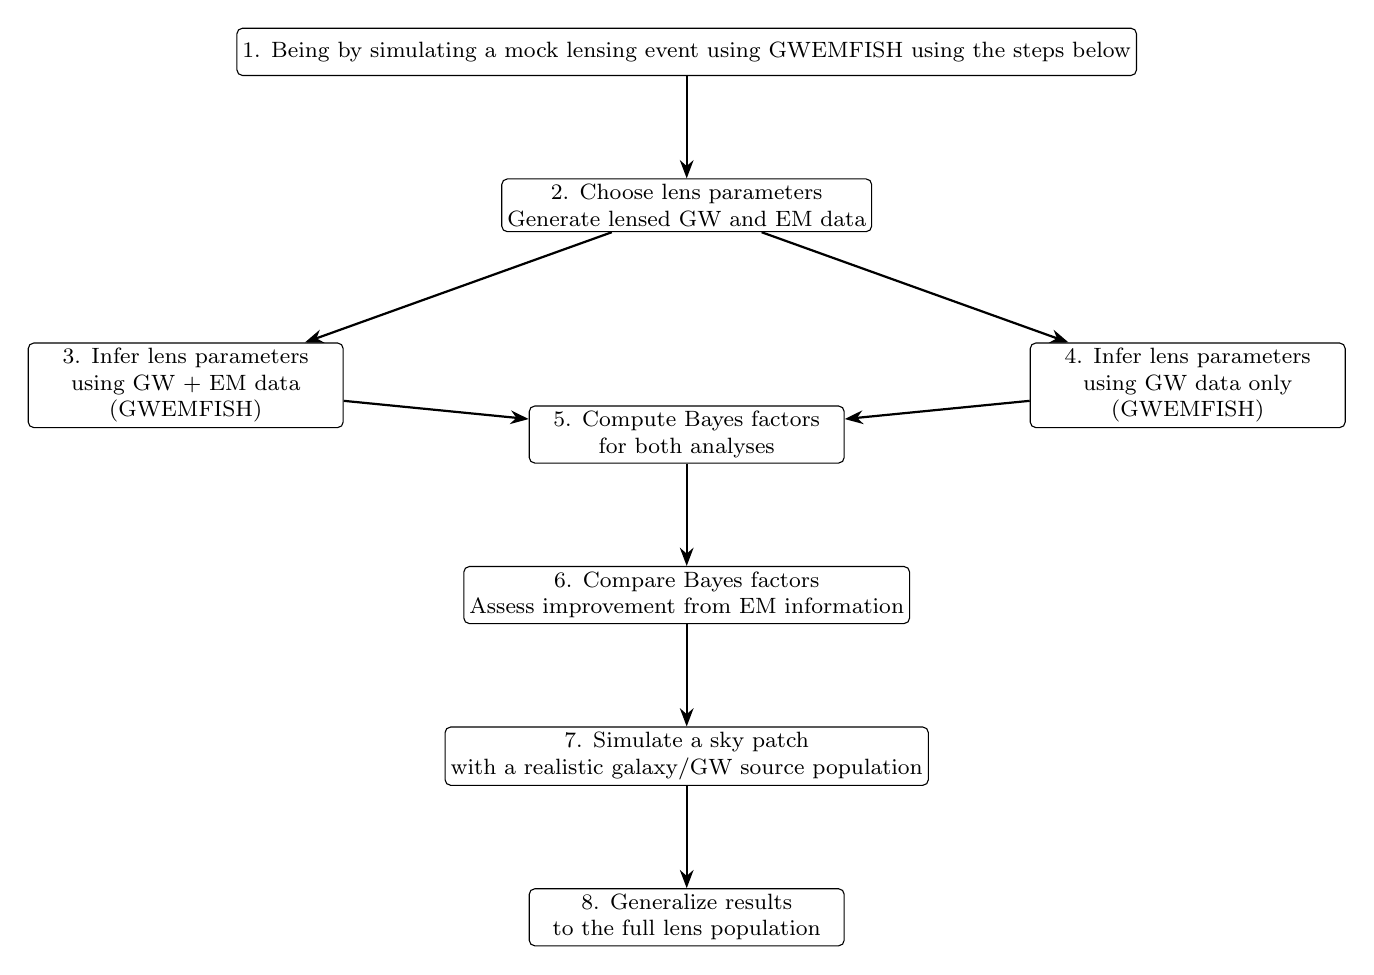
\begin{tikzpicture}[
    font=\footnotesize,
    node distance=1.3cm,
    >=Stealth,
    process/.style={
        rectangle,
        rounded corners=2pt,
        draw=black,
        align=center,
        minimum width=4cm,
        minimum height=0.6cm,
        inner sep=2pt
    },
    arrow/.style={->, thick}
]

% Nodes
\node (s1) [process] {1. Being by simulating a mock lensing event using GWEMFISH using the steps below};

\node (s2) [process, below=of s1]
{2. Choose lens parameters\\
Generate lensed GW and EM data};

\node (gwem) [process, below left=1.4cm and 2cm of s2]
{3. Infer lens parameters\\
using GW + EM data\\
(GWEMFISH)};

\node (gw) [process, below right=1.4cm and 2cm of s2]
{4. Infer lens parameters\\
using GW data only\\
(GWEMFISH)};

\node (bf) [process, below=2.2cm of s2]
{5. Compute Bayes factors\\
for both analyses};

\node (cmp) [process, below=of bf]
{6. Compare Bayes factors\\
Assess improvement from EM information};

\node (pop) [process, below=of cmp]
{7. Simulate a sky patch\\
with a realistic galaxy/GW source population};

\node (gen) [process, below=of pop]
{8. Generalize results\\
to the full lens population};

% Arrows
\draw [arrow] (s1) -- (s2);

\draw [arrow] (s2) -- (gwem);
\draw [arrow] (s2) -- (gw);

\draw [arrow] (gwem) -- (bf);
\draw [arrow] (gw) -- (bf);

\draw [arrow] (bf) -- (cmp);
\draw [arrow] (cmp) -- (pop);
\draw [arrow] (pop) -- (gen);

\end{tikzpicture}
\end{center}

\section{Schedule}

\begin{description}
	\item[Week 1] Introduction, set up, familiarize with terminal, and write up project plan
	\item[Week 2] Familiarize with GWEMFISH package, understand the relevant parameters, and attempt lens reconstruction on only one lens system and produce corner plots
	\item[Week 3] Be able to generate single lens reconstruction for both GW only and GW+EM
	\item[Week 4] Derive, finalize, and compute the Bayes factor to compare the difference between GW and GW+EM
	\item[Week 5] Generalize the result to a population of such systems
	\item[Week 6] tbd
	\item[Week 7] tbd
	\item[Week 8] tbd
\end{description}

\bibliography{sn-bibliography}% common bib file



\end{document}
